\documentclass[aspectratio=169,11pt]{beamer}

\usepackage[utf8]{inputenc}
\usepackage{amsmath}
\usepackage{booktabs}
\usepackage{ragged2e}

\usetheme{Madrid}
\usecolortheme{default}
\setbeamertemplate{navigation symbols}{}

\definecolor{NavyPrimary}{RGB}{16,42,67}
\definecolor{TealAccent}{RGB}{34,115,122}
\definecolor{LightGrayBg}{RGB}{245,247,250}
\definecolor{TextDark}{RGB}{35,35,35}

\setbeamercolor{normal text}{fg=TextDark,bg=white}
\setbeamercolor{title}{fg=white,bg=NavyPrimary}
\setbeamercolor{frametitle}{fg=white,bg=NavyPrimary}
\setbeamercolor{structure}{fg=NavyPrimary}
\setbeamercolor{section in toc}{fg=NavyPrimary}
\setbeamercolor{block title}{fg=white,bg=TealAccent}
\setbeamercolor{block body}{fg=TextDark,bg=LightGrayBg}
\setbeamercolor{item projected}{fg=white,bg=TealAccent}

\setbeamertemplate{blocks}[rounded][shadow=false]
\setbeamertemplate{footline}[frame number]
\setbeamertemplate{itemize item}{\color{TealAccent}$\blacktriangleright$}
\setbeamertemplate{itemize subitem}{\color{TealAccent}$\bullet$}

\addtobeamertemplate{frametitle}{}{%
  \vspace{-0.2em}\hspace{0em}\color{TealAccent}\rule{\paperwidth}{0.8pt}
}

\setlength{\parskip}{0.25em}

\title{Earnings Surprise, Firm Valuation, and Market Efficiency:\\Evidence from China}
\author{Corporate Finance Team Project\\[0.4em]\small Team Members: Yingqi Tan, Zhesheng Xu, Hao Yang}
\institute{FIN803 Corporate Finance}
\date{}

\begin{document}

\begin{frame}[plain]
  \titlepage
\end{frame}

\section{Introduction}

\begin{frame}{Motivation}
\begin{itemize}
  \item Earnings guidance updates expected future cash flows and should affect firm value.
  \item In semi-strong efficiency, public guidance information should be priced quickly.
  \item China A-share is a useful setting for testing whether pricing is immediate or delayed.
  \item The goal is not to maximize t-stats, but to estimate a defensible valuation-adjustment effect.
\end{itemize}
\end{frame}

\begin{frame}{Research Question}
\begin{block}{Core Question}
Do cleaner guidance-surprise signals predict post-announcement abnormal return in China A-shares?
\end{block}
\begin{itemize}
  \item Research question is unchanged.
  \item What changed is the empirical design: we now prefer a cleaner signal and a shorter event window.
  \item Final framing emphasizes limited short-run valuation adjustment, not strong long-run PEAD.
\end{itemize}
\end{frame}

\section{Theory}

\begin{frame}{Valuation Logic}
\begin{itemize}
  \item Firm value reflects discounted expected future cash flows.
  \item Guidance matters because it updates expected profitability.
  \item Prices should react to the surprise component relative to expectations, not to raw earnings news alone.
\end{itemize}
\end{frame}

\begin{frame}{Efficiency Interpretation}
\begin{itemize}
  \item Under semi-strong efficiency, public information should be incorporated quickly.
  \item If abnormal return appears shortly after announcement, that suggests incomplete immediate adjustment.
  \item But a long-window return pattern can be contaminated by unrelated news.
  \item So the identification strategy matters for how strong the inference can be.
\end{itemize}
\end{frame}

\section{Data and Design}

\begin{frame}{Sample and Events}
\begin{itemize}
  \item Sample period: 2020-01-01 to 2026-04-21.
  \item Test run shown here: 300 stocks, 5,162 raw guidance rows, 2,858 candidate events.
  \item Event types:
  \begin{itemize}
    \item guidance\_initial
    \item guidance\_upward\_revision
  \end{itemize}
  \item Event trading date: first trading day after announcement.
\end{itemize}
\end{frame}

\begin{frame}{Filtering and Tradability}
\begin{itemize}
  \item Exclude ST / *ST firms.
  \item Require at least 120 trading days since listing.
  \item Require tradable event-day return and non-zero event-day volume.
  \item Apply 20-day turnover-based liquidity filter.
  \item Purpose: reduce microstructure noise and make inference more credible.
\end{itemize}
\end{frame}

\begin{frame}{Why the Baseline Was Noisy}
\begin{itemize}
  \item Old signal \texttt{ES\_main} used a noisy proxy for expectations.
  \item Old headline outcome \texttt{CAR60} absorbed too much non-event information.
  \item Pooled long-window regressions were easy to over-interpret as strong PEAD.
  \item Group comparisons like ``moderate beats extreme'' were not stable enough to be the main conclusion.
\end{itemize}
\end{frame}

\begin{frame}{Why the Improved Specification Is More Defensible}
\begin{itemize}
  \item \texttt{ES\_std} better standardizes guidance surprise intensity.
  \item \texttt{CAR5} focuses on short-run valuation adjustment close to the announcement.
  \item Industry FE and year-quarter FE control for common shocks.
  \item Firm-clustered SE improve inference when firms appear repeatedly.
  \item This design is better suited to a cautious academic interpretation.
\end{itemize}
\end{frame}

\section{Variables and Methodology}

\begin{frame}{Preferred Variables}
\begin{itemize}
  \item Abnormal return: \(AR_{i,t}=R_{i,t}-R_{m,t}\)
  \item Preferred event window: \(CAR5 = \sum_{t=1}^{5} AR_{i,t}\)
  \item Preferred signal: \texttt{ES\_std}
  \item Controls: log size, beta
\end{itemize}
\begin{block}{Preferred Interpretation}
We test whether cleaner standardized surprise predicts short-run abnormal return, not whether large surprise mechanically implies strong long-run drift.
\end{block}
\end{frame}

\begin{frame}{Preferred Regression}
\[
CAR5_i = \alpha + \beta_1 ES\_std_i + \beta_2 \log(size_i) + \beta_3 beta_i + \text{Industry FE} + \text{YearQuarter FE} + \varepsilon_i
\]
\begin{itemize}
  \item Standard errors clustered by firm.
  \item Baseline CAR60 regression is retained only as a comparison benchmark.
\end{itemize}
\end{frame}

\section{Results}

\begin{frame}{Baseline vs Preferred Specification}
\begin{center}
\begin{tabular}{lcc}
\toprule
 & Baseline & Preferred \\
\midrule
Signal & ES\_main / moderate dummy & ES\_std \\
Outcome & CAR60 & CAR5 \\
Sample size & 2,375 & 2,529 \\
Key coefficient & 0.0225 & 0.00173 \\
p-value & 0.0481 & 0.0195 \\
Inference & clustered OLS & FE + clustered SE \\
\bottomrule
\end{tabular}
\end{center}
\vspace{0.5em}
\begin{itemize}
  \item Preferred specification is statistically cleaner, but the economic effect is modest.
\end{itemize}
\end{frame}

\begin{frame}{Preferred Main Result}
\begin{columns}[T,totalwidth=\textwidth]
\begin{column}{0.47\textwidth}
\begin{itemize}
  \item \texttt{ES\_std} coefficient on \texttt{CAR5}: 0.001732
  \item p-value: 0.0195
  \item Sample size: 2,529
  \item Interpretation: cleaner standardized surprise predicts modest short-run abnormal return.
\end{itemize}
\end{column}
\begin{column}{0.51\textwidth}
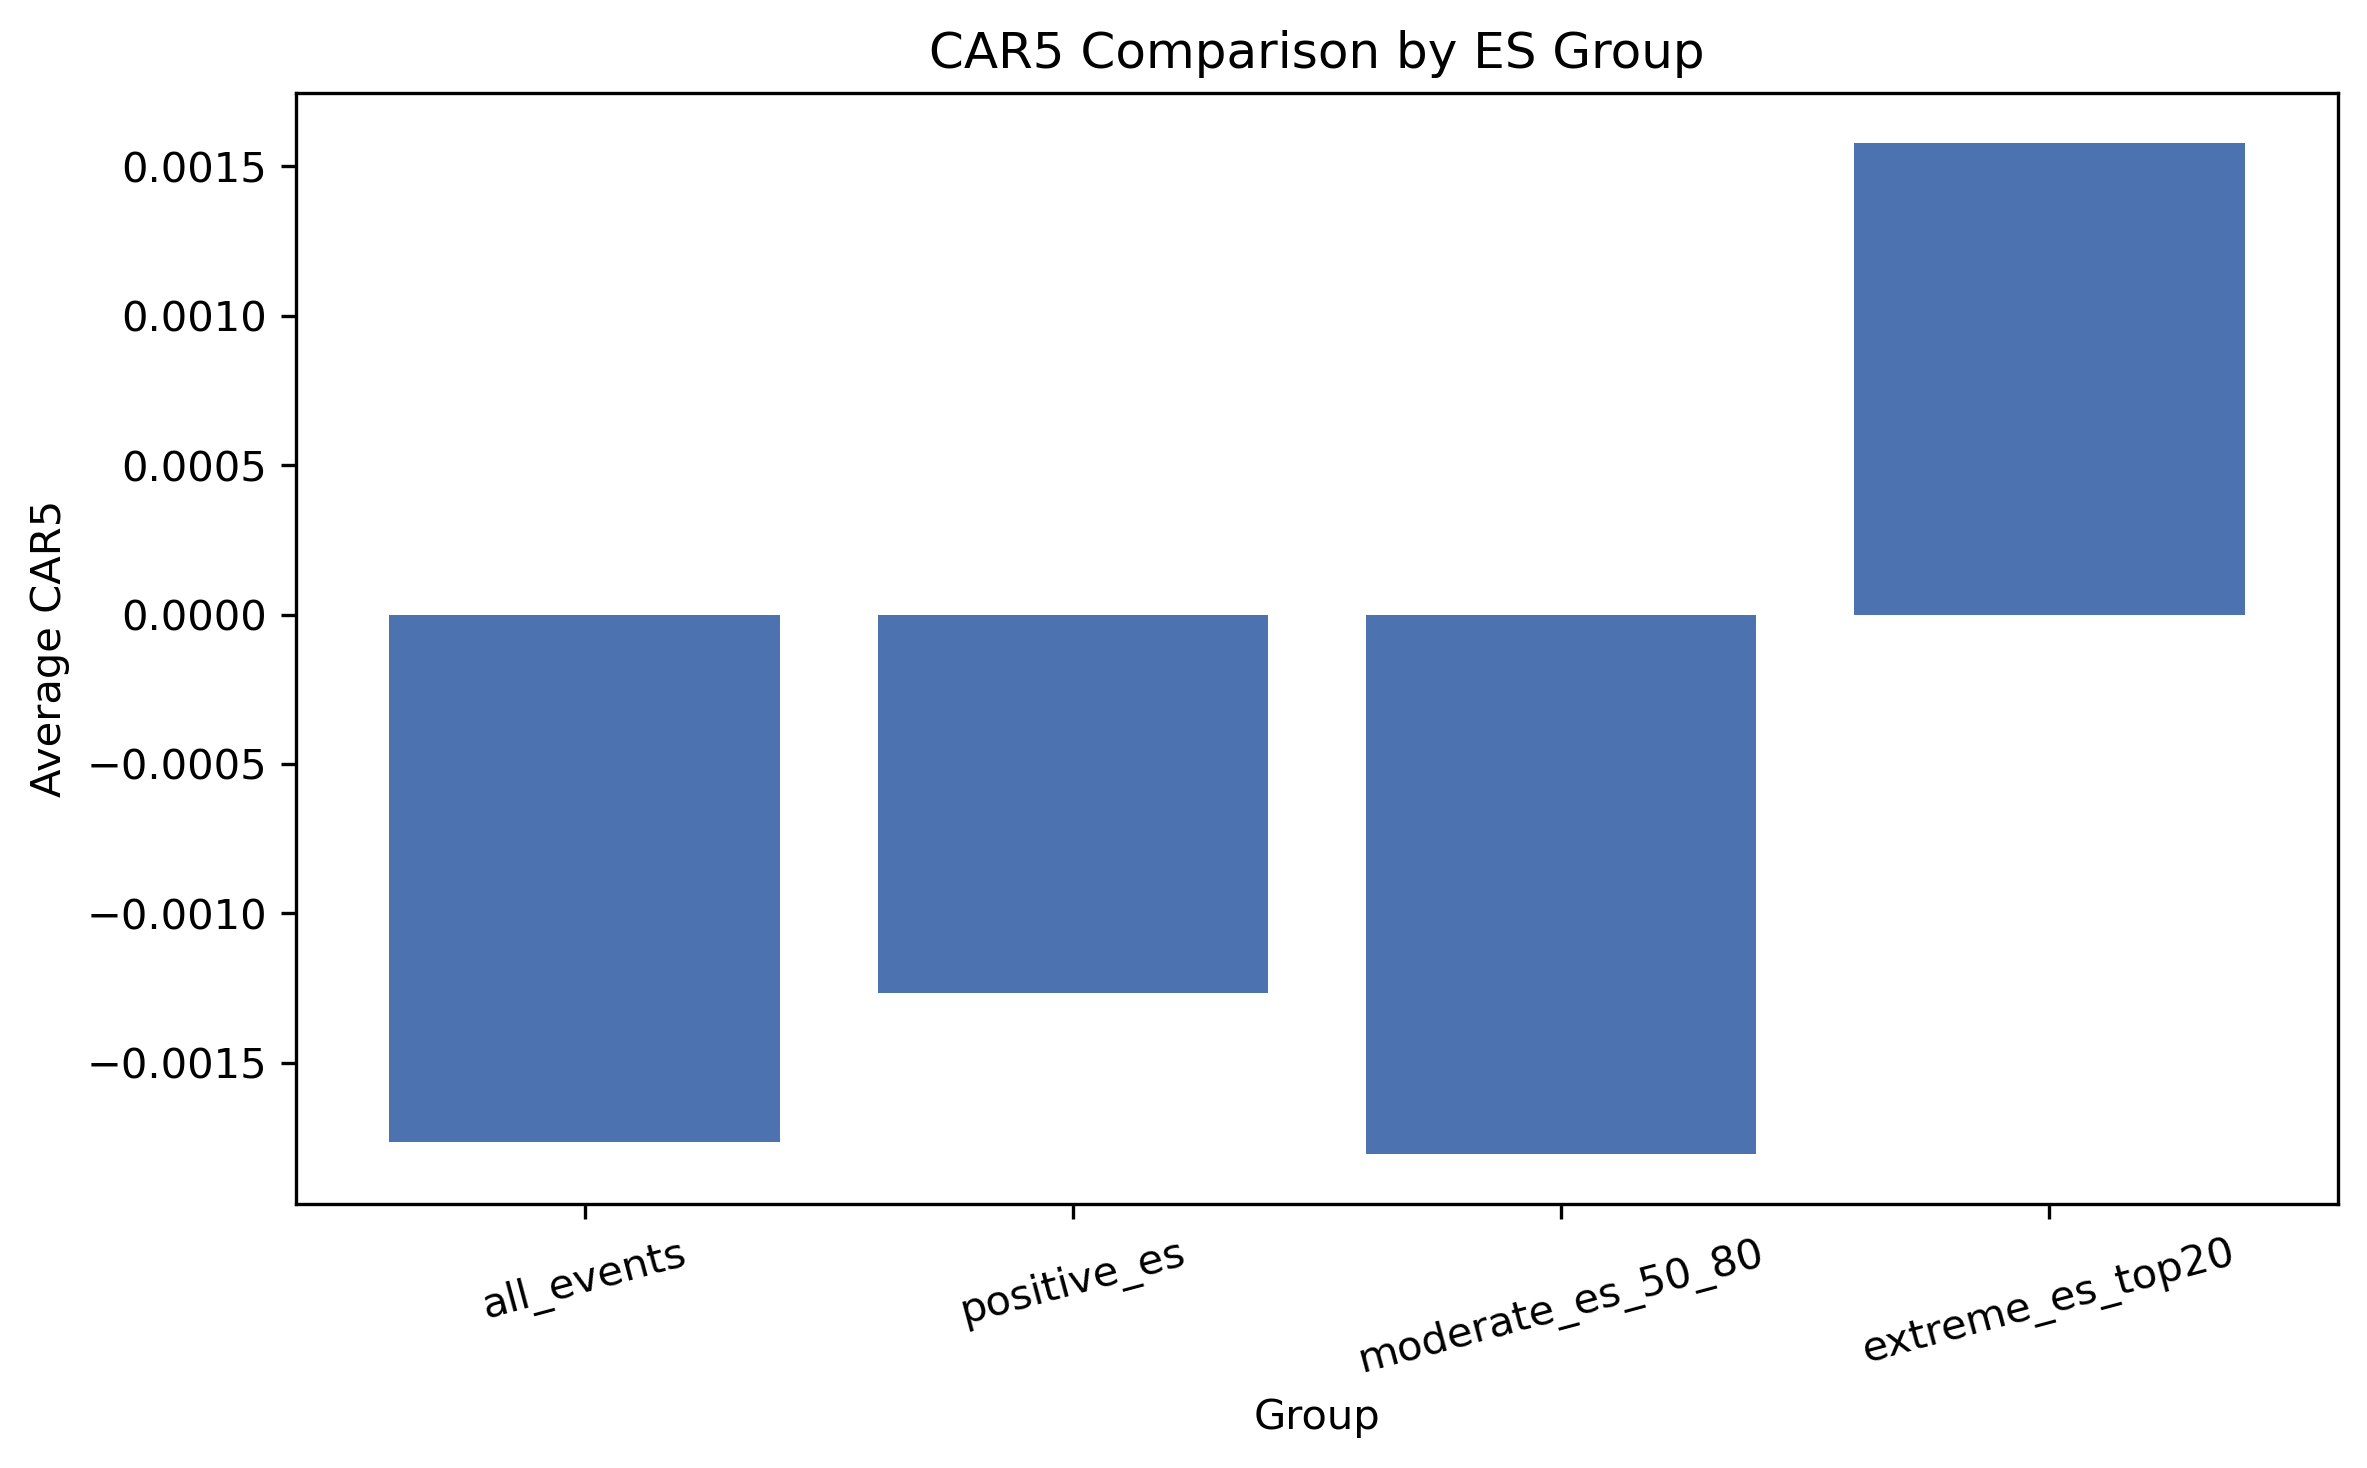
\includegraphics[width=\linewidth]{outputs/figures/fig1_es_group_comparison_improved.png}
\end{column}
\end{columns}
\end{frame}

\begin{frame}{Group Evidence Is Supplementary, Not Headline}
\begin{columns}[T,totalwidth=\textwidth]
\begin{column}{0.47\textwidth}
\begin{itemize}
  \item Improved group means at \texttt{CAR5} are small.
  \item Moderate group \texttt{CAR5}: about -0.18\%
  \item Extreme group \texttt{CAR5}: about 0.16\%
  \item So monotonic or dummy-group claims should not be the main narrative.
\end{itemize}
\end{column}
\begin{column}{0.51\textwidth}
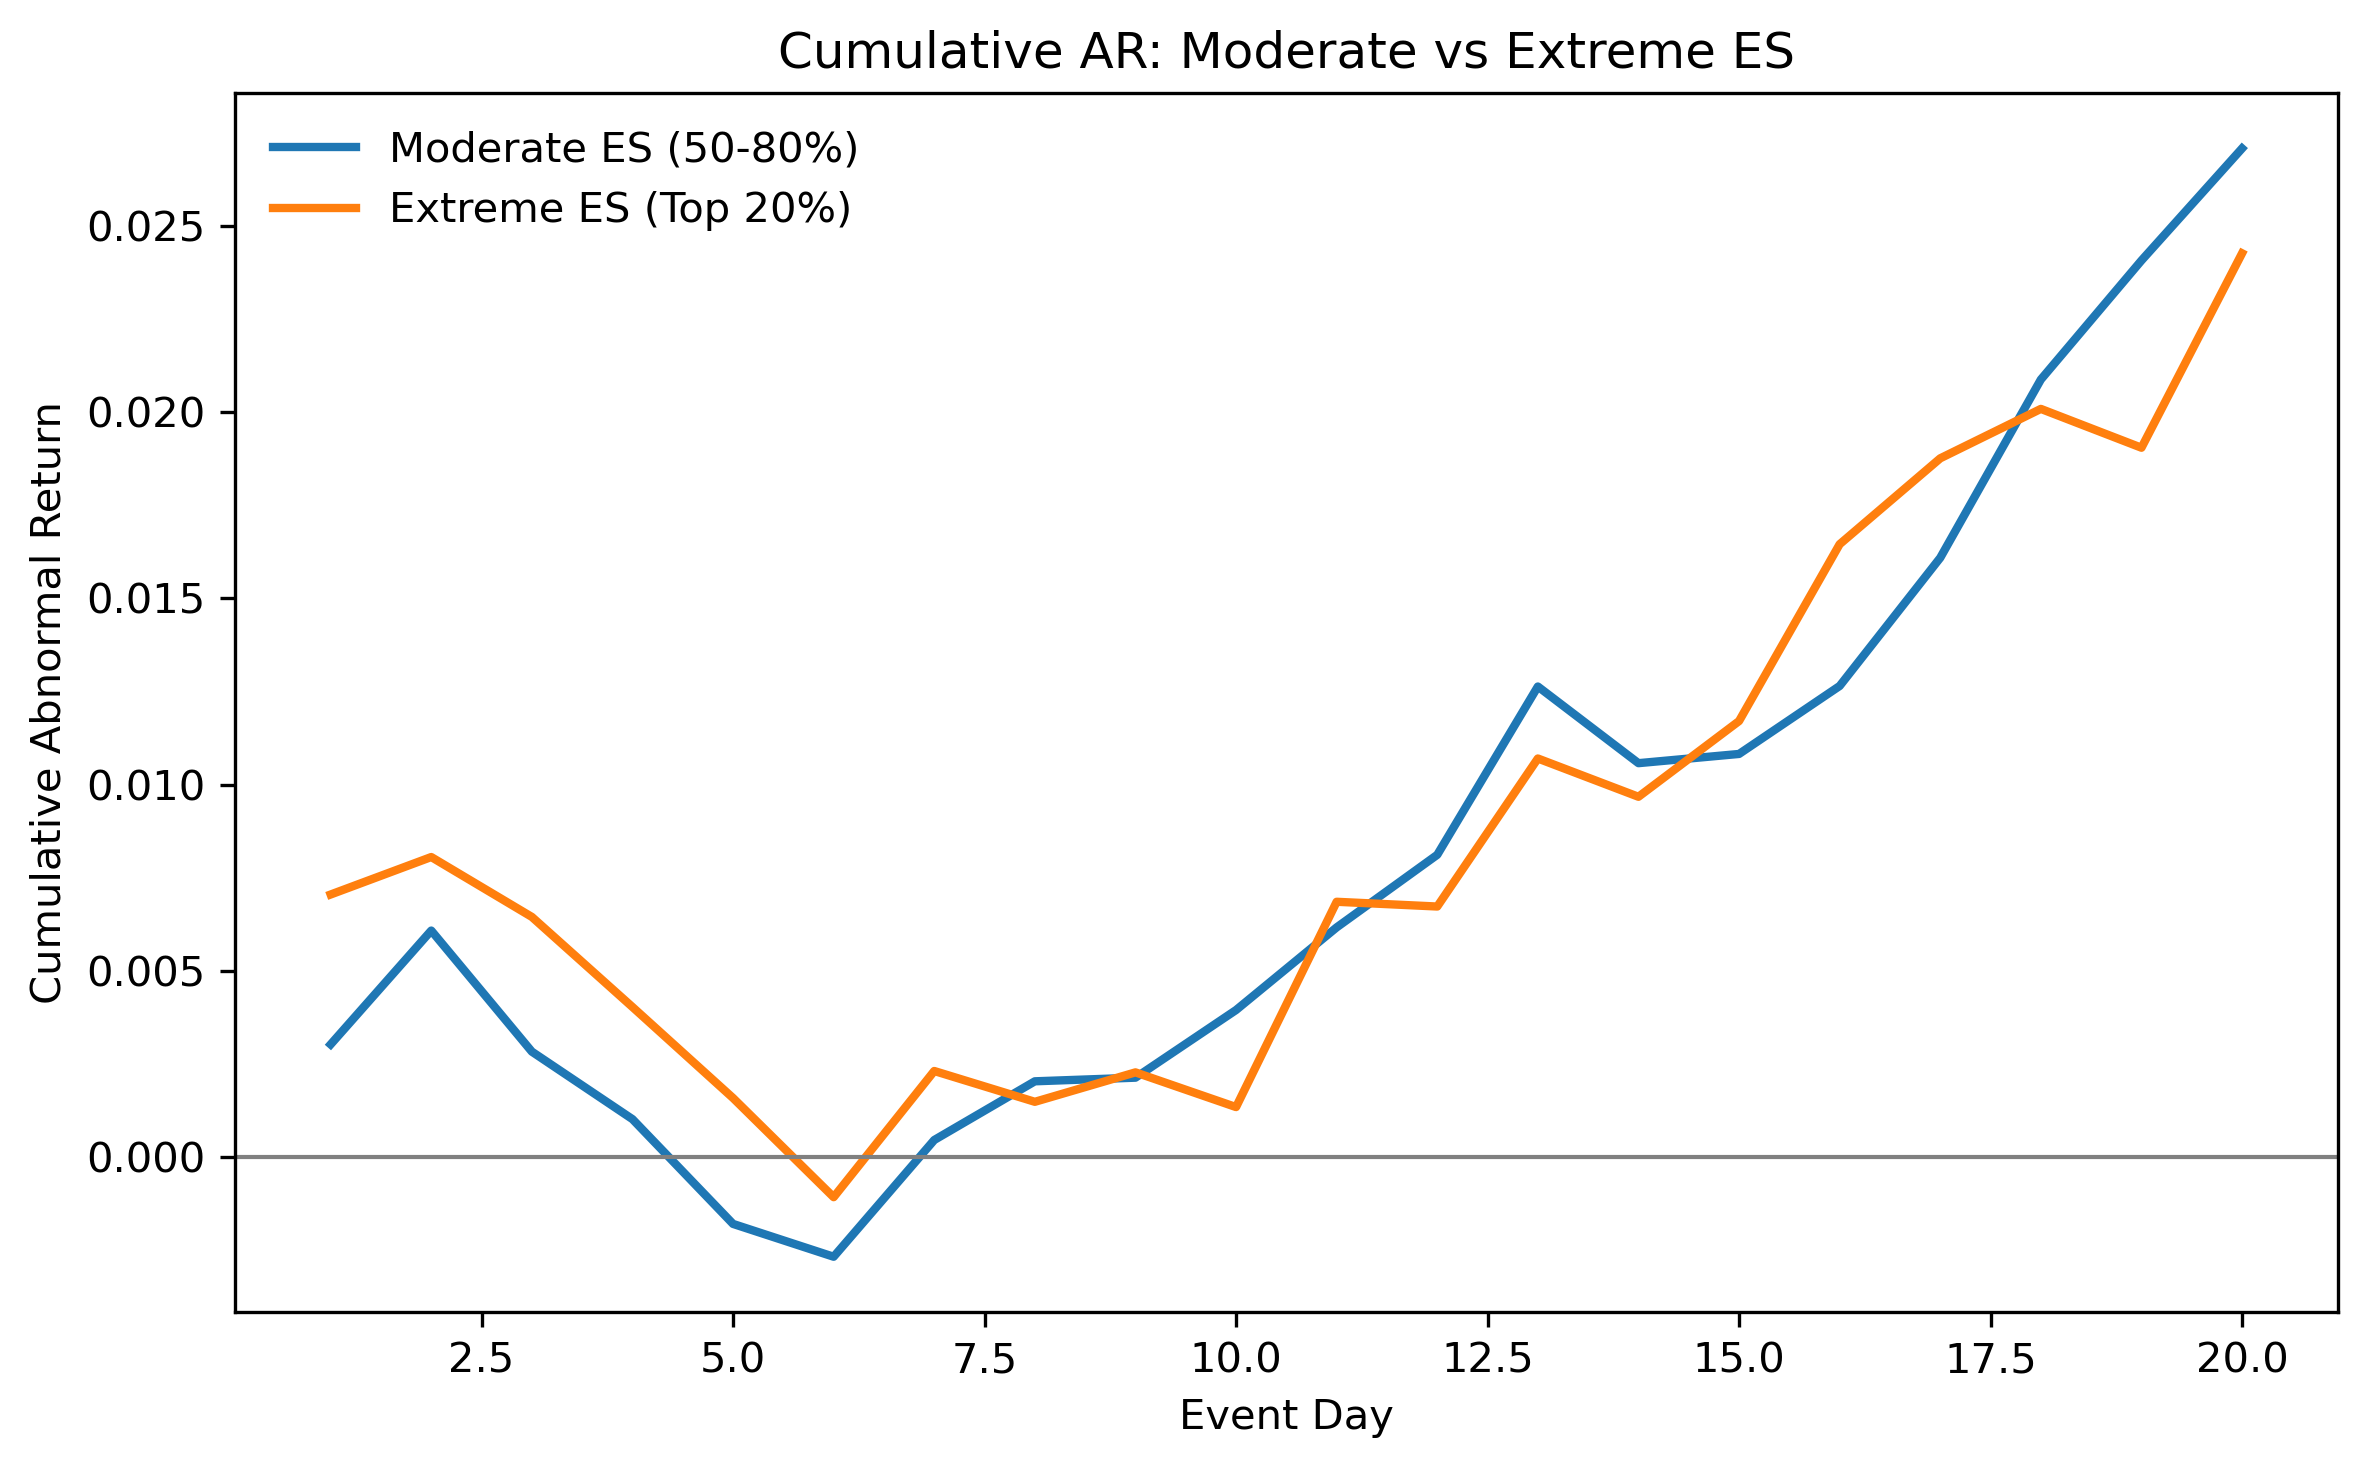
\includegraphics[width=\linewidth]{outputs/figures/fig2_cum_return_moderate_vs_extreme_improved.png}
\end{column}
\end{columns}
\end{frame}

\begin{frame}{Baseline as Robustness / Cautionary Comparison}
\begin{columns}[T,totalwidth=\textwidth]
\begin{column}{0.47\textwidth}
\begin{itemize}
  \item Baseline \texttt{CAR60} result remains positive and borderline significant.
  \item But long-window evidence is much easier to contaminate with later news.
  \item Therefore it should be treated as a robustness comparison, not the headline finding.
\end{itemize}
\end{column}
\begin{column}{0.51\textwidth}
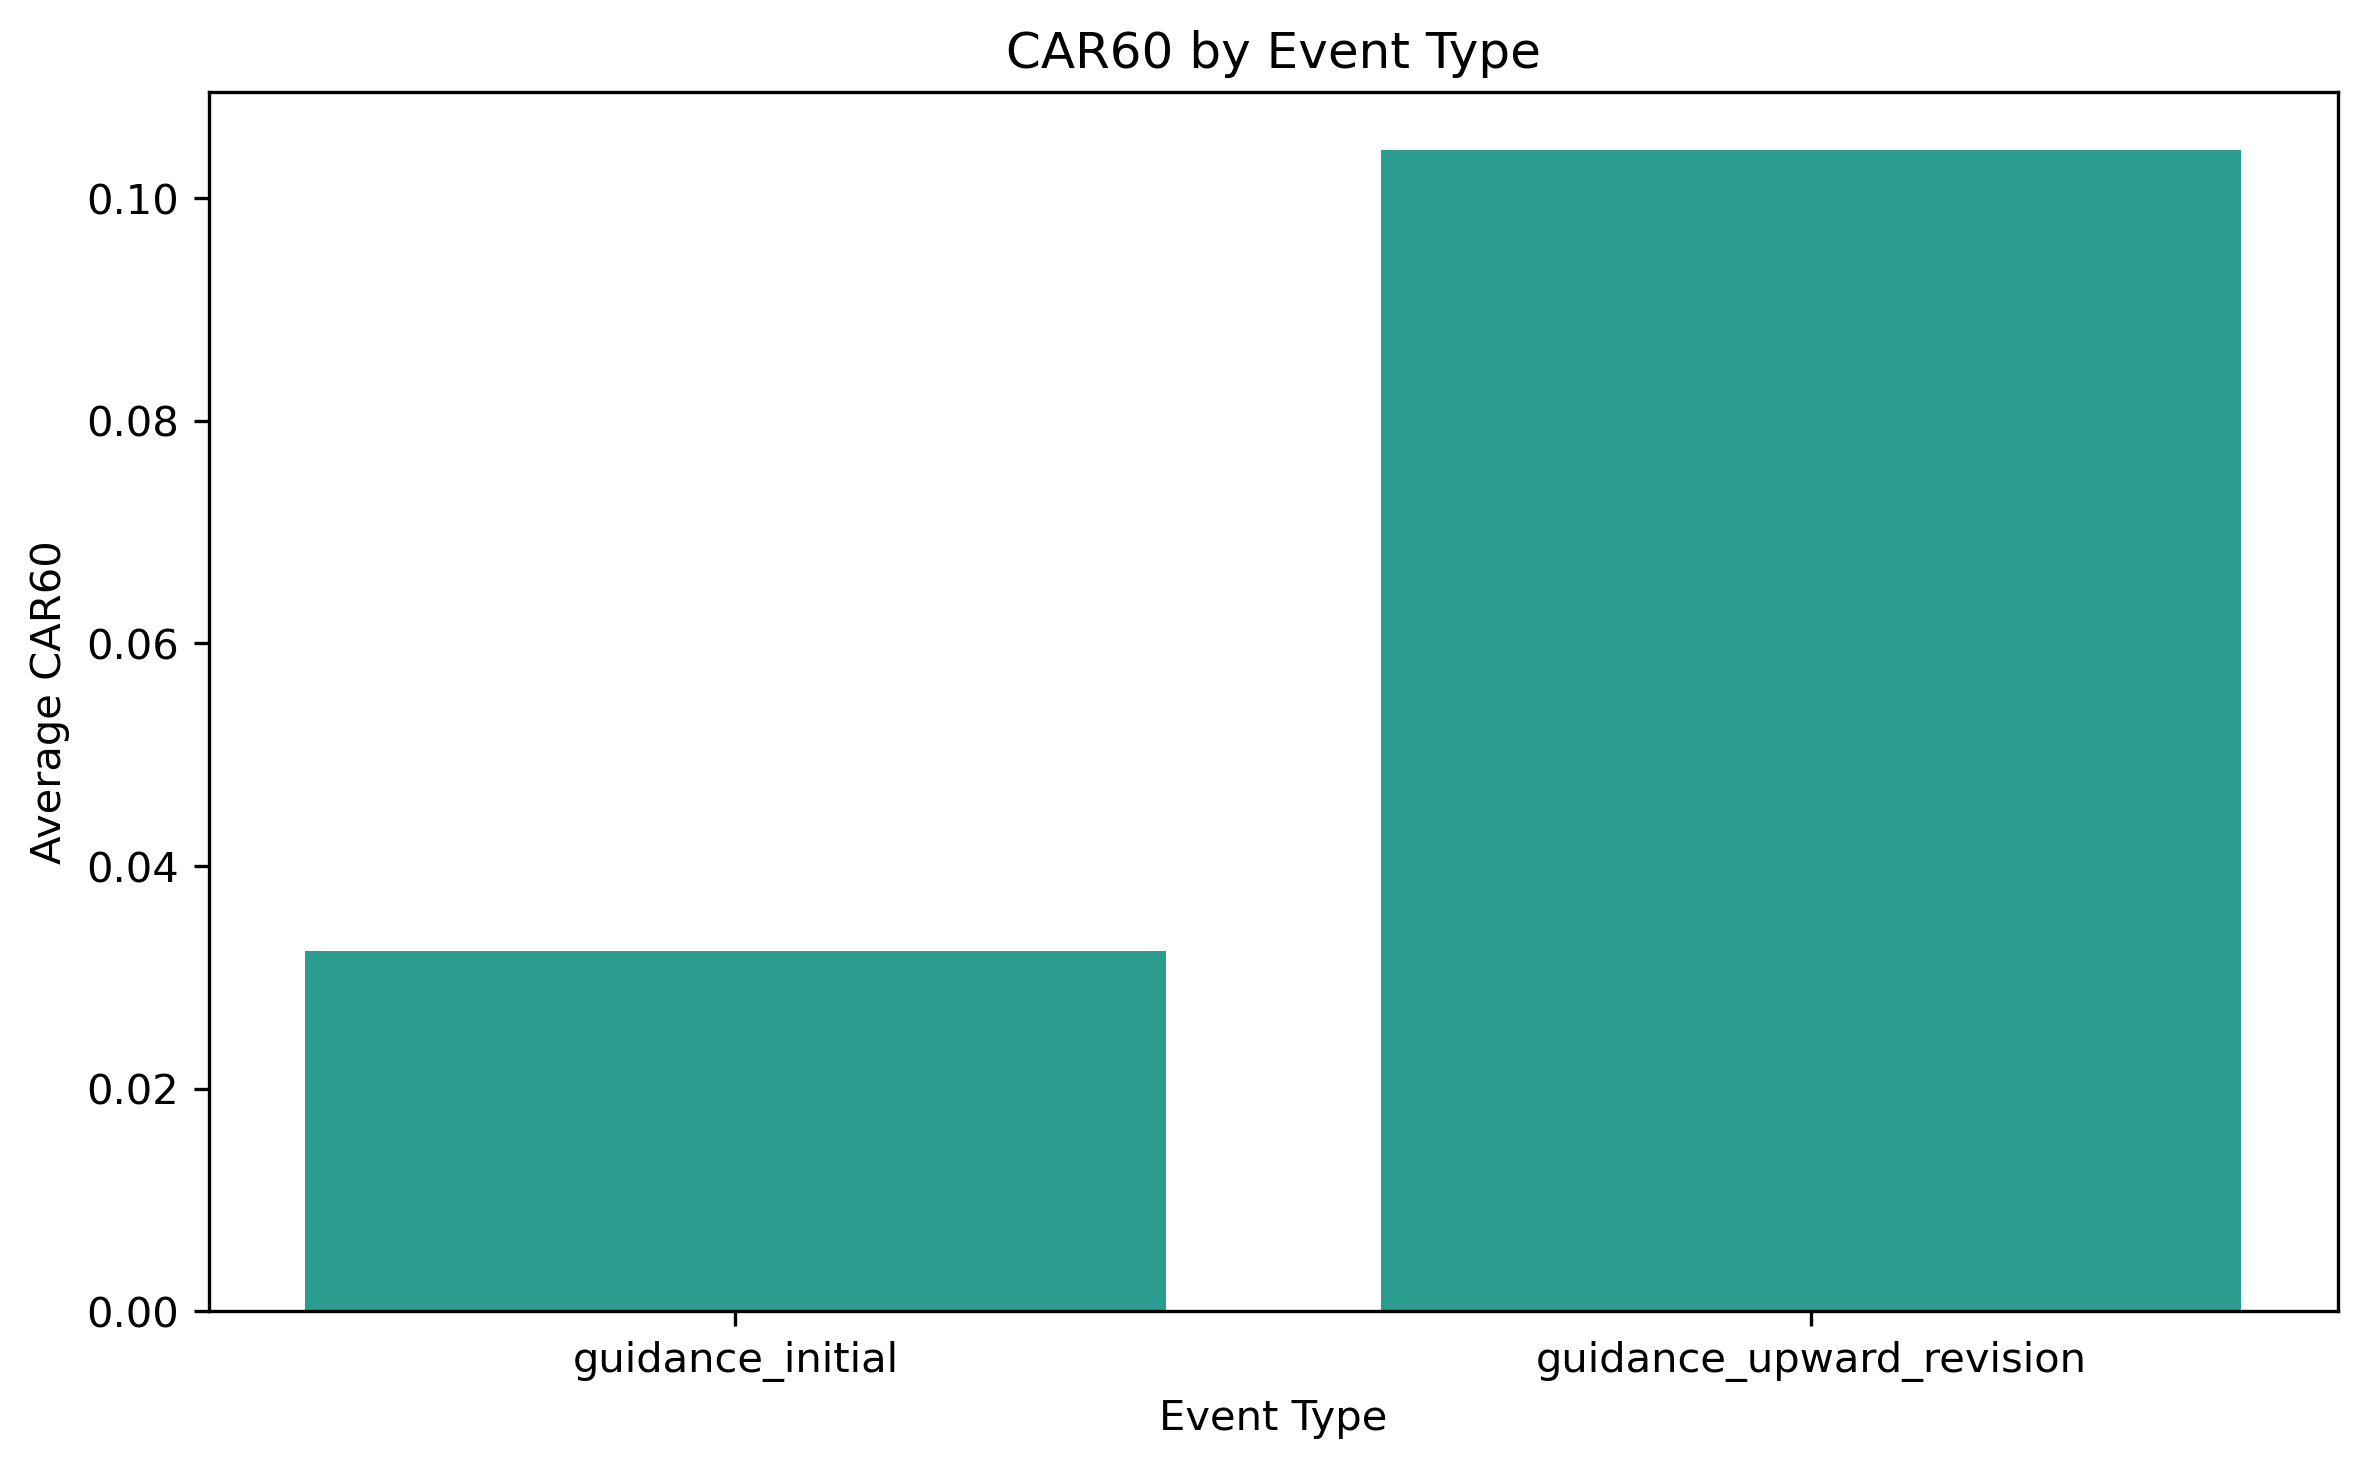
\includegraphics[width=\linewidth]{outputs/figures/fig3_event_type_comparison_baseline.png}
\end{column}
\end{columns}
\end{frame}

\section{Interpretation and Conclusion}

\begin{frame}{Corporate Finance Interpretation}
\begin{itemize}
  \item Guidance surprise affects valuation because it changes expectations about future profitability.
  \item The preferred evidence supports limited short-run underreaction, not a dramatic inefficiency story.
  \item Better signal construction matters as much as better regression design.
  \item The result is statistically meaningful, but economically modest.
\end{itemize}
\end{frame}

\begin{frame}{Final Conclusion}
\begin{itemize}
  \item Main result: cleaner standardized guidance surprise predicts modest but statistically significant short-run abnormal return.
  \item Best framing: limited short-run valuation adjustment after cleaner guidance surprise.
  \item Not supported as a headline claim: strong long-run PEAD, strong market inefficiency, or stable monotonic group ordering.
  \item Next step: improve the expectation benchmark further with better analyst-consensus data.
\end{itemize}
\end{frame}

\end{document}
